\chapter{Bouwstenen tekstanalyse}\label{Lectuur}

In dit hoofdstuk wordt de theoretische achtergrond en de keuze voor de technieken die we gebruiken tijdens het experiment toegelicht. We bespreken in \ref{Voorstelling dataset} de gebruikte voorstelling van de dataset. In \ref{Technieken voor Pre-Processing} bespreken we enkele optimalisatie technieken die kunnen helpen om de classificatieprestaties te verbeteren. Daarna volgen in \ref{Leermethode} de zelflerende algoritmes zelf, waarin de werking van en de keuze voor de algoritmes wordt uitgelegd. 

\section{Overzicht}\label{Overzicht}

\section{Voorstelling dataset}\label{Voorstelling dataset}
%
De voorstelling van de data is een eerste element van het experiment waarmee men rekening moet houden. We kunnen bijvoorbeeld rauwe data meegeven aan het zelflerende algoritme of we kunnen de tekst omvormen naar een vector die het aantal voorkomens van ieder woord in de tekst bevat. Voor het experiment kiezen we het tweede voorbeeld, waarbij we een document voorstellen als een vector met daarin de woordfrequentie. Dit wordt de vector space methode genoemd en wordt door \cite{turney2010frequency} beschouwd als onderdeel van de oplossing voor de problematiek rond semantische analyse. Verder is deze voorstelling een populaire methode binnen het onderzoek naar gevoelsanalyse op het Engels en heeft dit zijn werking al aangetoond. Zie bijvoorbeeld \cite{pang2002thumbs} en \cite{maas2011learnin}.

\subsection{Vector Space Methode}\label{Vector Space Methode}
%
De vector space methode (VSM) is een methode waarbij we een document als een vector voorstellen waarbij ieder element overeenkomt met een woord en zijn frequentie in het document. De elementen van de vector worden ook wel features genoemd. 
Als men concreet een document voorstelt kan men zeggen dat document $j$ voorgesteld wordt door $d_{j}$ met $f_{ij}$ de frequentie van het woord $w_{i}$. Met de frequentie $f_{ij}$ bedoelt men het totaal aantal voorkomens van het woord $w_{i}$ in document $j$. Het aantal verschillende woorden in het document stelt men voor door $n_{w}$, wat eveneens de dimensie is van de vector.
Het document $j$ kan dus als volgt worden voorgesteld:
%
\[ d_{j}  = \begin{bmatrix}
    f_{1j} \\
    f_{2j} \\
    \vdots \\
    f_{n_{w}j} \\
\end{bmatrix}  
\]
%
Een belangrijk inzicht bij de vector space methode is dat een document voorgesteld wordt als een groep van woorden. Er wordt geen rekening gehouden met de volgorde waarin de woorden in het document voorkomen. Vaak ziet men ook dat de vector vaak ijl is en vanwege de grote hoeveelheid aan woorden in een document heel groot. Als we nu niet \'e\'en document, maar meerdere documenten nemen en we zeggen dat het aantal documenten gelijk is aan $n_{d}$, resulteert dit in een matrix waarbij iedere kolom een document voorstelt.
\[
D =
 \stackrel{\mbox{Documenten}}{%
    \begin{bmatrix}
    f_{11} & f_{12} & \cdots & f_{1n_{d}} \\
    f_{21} & f_{22} & \cdots & f_{2n_{d}} \\
    \vdots & \vdots & \ddots & \vdots \\
    f_{n_{w}j} & f_{n_{w}2} & \cdots & f_{n_{w}n_{d}}
    \end{bmatrix}
    }
    & Woorden \]
%
Deze matrix wordt een \textbf{\textit{terms-documents matrix (TDM)}} genoemd. Wanneer men spreekt van een \textbf{\textit{documents-terms matrix (DTM)}}, spreekt men een getransponeerde terms-documents matrix. Een rij van een DTM stelt dan een document voor. In het experiment stellen we onze data voor aan de hand van een documents-terms matrix
%
De voorstelling in een matrix geeft inzicht en biedt veel meer mogelijkheden om de data te analyseren. Bijvoorbeeld overeenkomstige woordfrequenties tussen twee documenten kan duiden dat documenten over hetzelfde onderwerp gaan of eenzelfde mening uitdrukken.
%
In de praktijk is gebleken dat documenten vergelijken op basis van woordfrequentie niet altijd de gewenste resultaten oplevert en \cite{pang2002thumbs} toont aan dat er ruimte is voor verbetering door middel van Pre-Processing technieken.

\section{Technieken voor Pre-Processing}\label{Technieken voor Pre-Processing}

Zoals we in \ref{Vector Space Methode} al vermeldde kan pre-processing voor verbetering van de classifiers zorgen. De pre-pocestechnieken die we gebruiken in deze bachelorproef zijn al eerder gebruikt door \cite{pang2002thumbs} en \cite{wang2011sentiment} en hadden een positief effect.

\subsection{Bag of Words}\label{Bag of Words}

De eerste techniek is Bag of Words. Dit is niet echt een pre-procestechniek, maar eerder een referentiepunt voor de andere pre-procestechnieken. Het steunt op het principe waarop de vector space methode zich baseert, waarbij ieder document wordt voorgesteld door zijn woordfrequenties. Het is de basistechniek die wordt uitgevoerd bij een gevoelsanalyse aan de hand van de VSM. 

\subsection{Verwijderen van stopwoorden}\label{Verwijderen van stopwoorden en leestekens}

Wat men vaak ziet in het Nederlands, maar ook in taal algemeen, is dat er veel stopwoorden worden gebruikt. Stopwoorden als ``klopt'' en ``eigenlijk'' zeggen niet veel over teksten of ze nu positief of negatief zijn. Als een bepaald woord niet bijdraagt voor het algoritme kunnen we stopwoorden beschouwen als ruis in de dataset. Ruis vertroebelt het beeld van het concept dat we het algoritme willen aanleren en proberen we te elimineren. Daarom beschouwt men het verwijderen van stopwoorden en leestekens ook als een manier van pre-processing.

\subsection{Term weighting}\label{Term weighting}

Als we terugkijken naar de vector space methode, waarbij we enkel rekening houden met de woordfrequentie, kan men zeggen dat niet elk woord evenveel doorweegt. Een woord dat in alle documenten voorkomt biedt geen of minder waardevolle informatie, dan een woord dat zelden voorkomt. En hierop baseert term weighting zich. Het gaat een wegingsfactor introduceren. Ieder woord krijgt een gewicht toegewezen, dat weergeeft hoe belangrijk het woord is. Neem als voorbeeld een hoop recensies van de film ``Pulp Fiction'' en de woorden ``Pulp'' en ``excellent''. ``Pulp'' is een woord dat voorkomt in de titel van de film en komt ongetwijfeld in elke recensie voor. ``Excellent'' daarentegen is een woord dat enkel maar voorkomt wanneer de recensent de film fantastisch vond, het zal niet in elk document voorkomen en is waardevolle informatie. Term weighting zal dus bij dit voorbeeld ``excellent'' een groter gewicht toewijzen dan ``Pulp''. 
%
De kwantiteit van dit gewicht wordt vaak de \textbf{inverse document frequency  (idf)} genoemd en wordt bepaald aan de hand van volgende formule:
\[w_{i}: idf_{i} = -log_{2}[P(w_{i})] \]
met $P(w_{i})$ de priori probability dat woord $w_{i}$ voorkomt in het document.\\
%
De inverse document frequency geeft het algemeen belang van het woord $w_{i}$ weer. Men kan dit benaderen door het logaritme te nemen van het aantal documenten waar $w_{i}$ in voorkomt en het totaal aantal documenten.
Een andere nuttige kwantiteit is de  \textbf{term frequency} $tf_{ij}$. Deze geeft het belang weer van het woord $w_{i}$ binnen in het document $d_{j}$  en wordt als volgt genoteerd:
\[ tf_{ij} = \frac{f_{ij}}{ \sum_{i=1}^{n_{w}}f_{ij}} \]
%
$tf_{ij}$ wordt berekend door de frequentie, het aantal voorkomens, van een woord $w_{i}$ in document $d_{j}$ te delen door de som van alle woordfrequenties in document $d_{j}$.
Met deze twee kwantiteiten kan men een nieuwe begrip introduceren: de \textbf{tf-idf score}. Wat overeenkomt met het product van tf en idf.
\[ \text{tf-idf score} = tf . idf_{ij} = idf_{i} . tf_{ij} \]
%
De tf-idf matrix bekomt men dan door alle woordfrequenties van het terms-document matrix te vervangen door de tf-idf score.
Er bestaan nog uitbreiding op term weighting (\cite{altoglou2010study}), maar voor het experiment houden we het bij de standaard tf-idf weighting.


\subsection{Bigram Collocaties}\label{Bigram Collocaties}

Bigrams Collocaties is een techniek waarbij men op zoek gaat naar paren van woorden die een hoge waarschijnlijkheid hebben om samen voor te komen en een extra bron van informatie kunnen vormen. In het onderzoek van \cite{pang2002thumbs} bleken bigrams niet voor een verbeterde prestatie te zorgen, al mag men de nuttigheid van bigrams niet onderschatten. Toch nemen we bigrams als een van de technieken,\cite{edersen2001decision} toonde echter aan dat bigrams een nuttig kenmerk vormen voor het oplossen van woord zin ambiguïteit. \cite{pang2002thumbs} merkt dan ook zelf op in zijn onderzoek dat bigram features mogelijks evenwaardig zijn met unigram features.\\
%
De bepaling van de informatieve waarde van de bigrams is gebaseerd op de frequentie van het bigram en de frequenties van de andere bigrams. Als men een overzicht krijgt over de frequenties introduceert men een metriek, die met behulp van de frequenties mogelijke verbanden kan blootleggen. Chi-kwadraat is zo'n metriek die er zich toe leent. De Chi-kwadraattoets is een statistische toets die het mogelijk maakt om de onafhankelijkheid tussen waarnemingen te onderzoeken. Bij Bigram Collocaties onderzoekt men via de Chi-kwadraattoets de afhankelijkheid tussen twee woorden. Hoe grotere de afhankelijkheid, hoe hoger de score.   

\subsubsection{Chi-Kwadraattoets}\label{Chi-Kwadraattoest}

De Chi-Kwadraattoets is een techniek uit de statistiek die gebruikt  kan worden als een onafhankelijkheidstoets voor waarnemingen. De reden waarom we deze toets voor Bigram collocatie gebruiken is dat de toets parametervrij is. Wat wil zeggen dat er bij de start van de chi-kwadraattoets geen aanname over de populatie of het gemiddelde wordt verwacht. In deze sectie leggen we aan de hand van een voorbeeld uit hoe de chi-kwadraattoets juist deze afhankelijkheid bepaald.\\
%
Neem als voorbeeld het bigram \textit{(heel , goed)}. Zoals bij iedere statistische test neemt men eerst een nulhypothese aan. Voor de chi-kwadraattoets is dit ook het geval. De toets neemt als nulhypothese aan dat beide woorden onafhankelijk van elkaar zijn en elkaars voorkomen niet be\"invloeden. Men vergelijkt de waargenomen frequenties van de woorden met de verwachte frequenties wanneer de woorden onafhankelijk zouden zijn. Als deze waarden te veel verschillen kan men de nulhypothese verwerpen en de alternatieve hypothese aannemen, namelijk dat de woorden afhankelijk zijn van elkaar. \\
\newline
%
Om de afhankelijkheid van woorden te bepalen, kijken we naar volgende gegevens:
\begin{itemize}
  \item het aantal voorkomens van het woord in een bigram
  \item het aantal voorkomens van het woord in een bigram met het ander woord waar we de afhankelijkheid van onderzoeken
  \item het totaal aantal bigrams
  \item het aantal voorkomens van het ander woord in een bigram. 
\end{itemize}
%
%
Als we voor het voorbeeld \textit{(heel , goed)} bovenstaande gegevens in een kruistabel gieten krijgen we de volgende 2x2 tabel:
\begin{table}[h!]
\centering
\begin{tabular}{|l|c|r|}
\hline
          & w1= heel                                                         & w1 $\neq$ heel                                                                \\ \hline
w2 = goed & \begin{tabular}[c]{@{}c@{}}9\\ (heel goed)\end{tabular}          & \begin{tabular}[c]{@{}r@{}}7893\\ (bv. niet goed)\end{tabular}           \\ \hline
w2 $\neq$ goed & \begin{tabular}[c]{@{}c@{}}3632\\ (bv. heel slecht)\end{tabular} & \begin{tabular}[c]{@{}r@{}}13498000\\ (bv. boeiende thesis)\end{tabular} \\ \hline
\end{tabular}
\end{table}
\newline
We weten nu naar wat we moeten kijken bij het analyseren van de afhankelijkheid maar er mist nog een weging, een onderlinge verhouding tussen de kenmerken. 
%
De Chi-Kwadraatsom biedt hier de oplossingen en geeft die weging. De toetsingsgrootheid voor de Chi-kwadraattoets wordt gedefinieerd aan de hand van de volgende formule:

\[{\chi}^2=\sum_{i,j}^{} \frac{(O_ij - E_ij)^2}{E_ij}\]
%
Waarbij ${O_ij}$ het aantal keer dat het paar $(i,j)$ voorkomt. $E_ij$ stelt de voorspelde waarden voor als de woorden onafhankelijk moesten voorkomen\\
$E_ij$ wordt bepaald door volgende formule:

\[{E_ij}= \frac{O_i*}{N} + \frac{O_*j}{N} * N = \frac{O_i* O_*j}{N} \]
%
met $\frac{O_i*}{N}$ de marginale probabiliteit dat $i$ als eerste deel van het bigram voorkomt en $\frac{O_j*}{N}$ de marginale probabiliteit dat $j$ als tweede deel van het bigram voorkomt. $N$ stelt het totaal aantal bigrams voor.
%
Toegepast op het voorbeeld geeft dit voor het bigram ``(heel , goed)'':

\[{E_11} = \frac{9+3632}{N}+\frac{9+7893}{N} * N \approx 0,0085 \]
\newline
Als laatste onderdeel berekenen we de ${\chi}^2$-score, bepalen we het aantal vrijheidsgraden en zoeken we de ${\chi}^2$ distributie op met de berekende vrijheidsgraad. Stel dat het vooropgestelde betrouwbaarheidsinterval 95\% bedraagt dan kunnen we de kritische waarde bepalen voor significantielevel $\alpha$ = 0,005.
Als de berekende ${\chi}^2$-score in het verwerpingsgebied ligt, kan de nulhypothese verworpen worden en kan het bigram beschouwd worden als afhankelijk.\\
%
Onderstaande afbeelding illustreert hoe de verwerping of aanvaarding van een nulhypothese juist in zijn werking gaat
%
\begin{figure}[h]%
    \centering
    \subfloat{{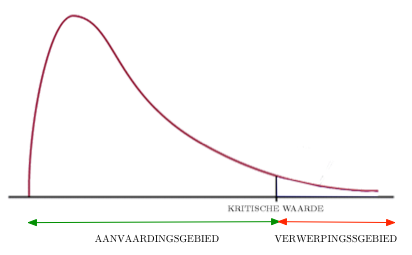
\includegraphics[width=10cm]{confidence_interval_chi_square} }}%
    \caption{Illustratie eenzijdige-toets van een ${\chi}^2$-distributie (Originele afbeelding: http://www.philender.com/courses/intro/notes3/xdist.gif)}%
\end{figure}
\newline
Kort samengevat baseert de Chi-kwadraattoets zich op de afwijking tussen de geobserveerde frequentie en de verwachte frequentie. Hoe groter het verschil, hoe waarschijnlijker men de nulhypothese kan verwerpen. En dit is waar men zich bij Bigram Collocatie op gaat baseren.

\begin{figure}[h]%
    \centering
    \subfloat{{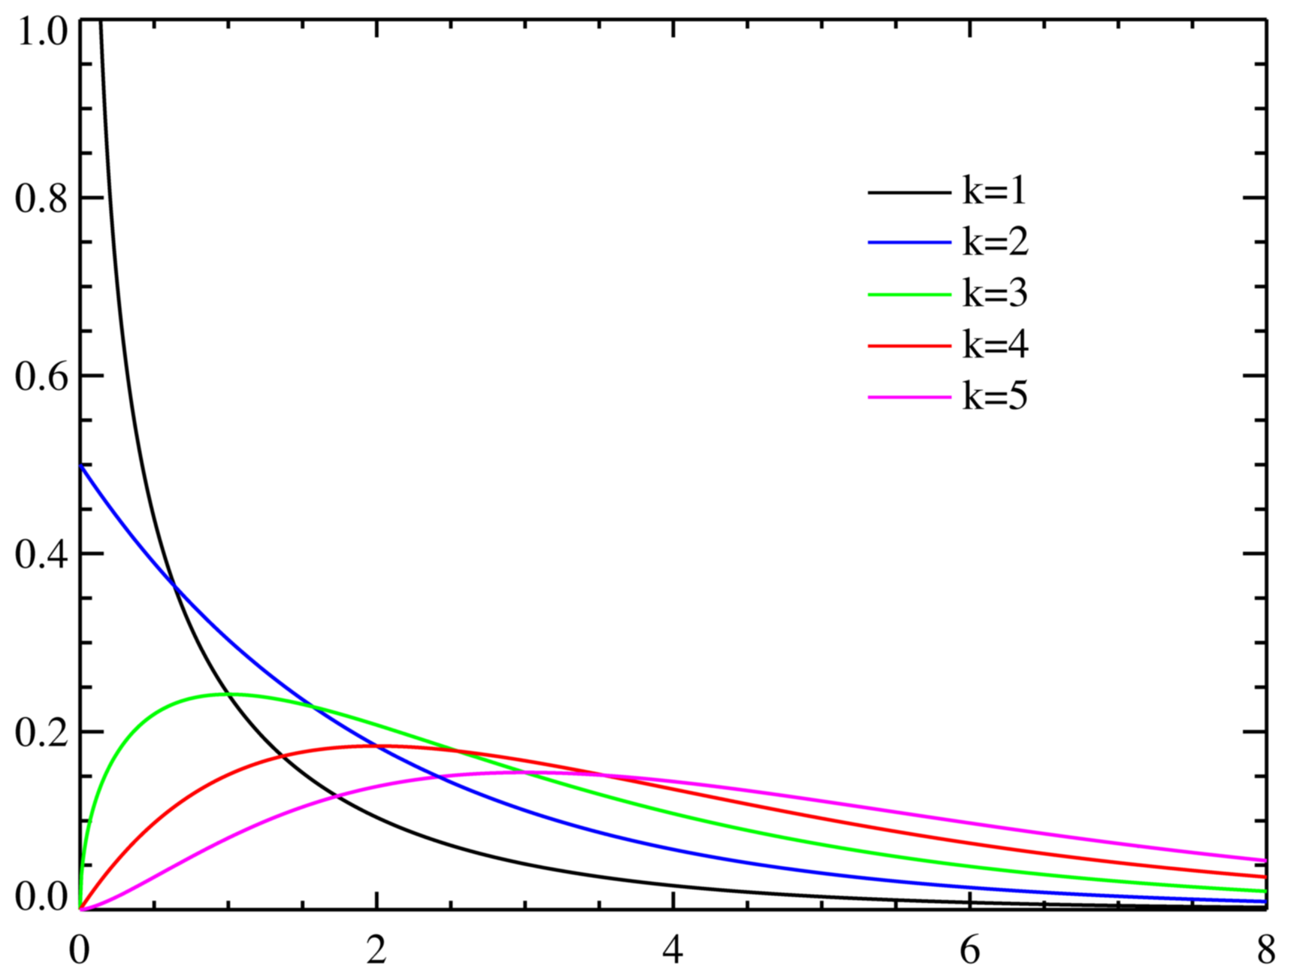
\includegraphics[width=6cm]{Chi-square_distribution} }}%
    \caption{Chi-square distributies met K vrijheidsgraden (Bron: \url{http://upload.wikimedia.org/wikipedia/commons/2/21/Chi-square_distributionPDF.png})}%
\end{figure}

\subsection{Best feature selection}\label{Low-information feature el}

Als we duizenden documenten verwerken, is het te voorspellen dat er enorm veel woorden algemeen voorkomen in de documenten, maar niet veel informatie bijdragen over het document zelf. Het is sterk vergelijkbaar met de voorgaande techniek in \ref{Verwijderen van stopwoorden en leestekens} bij het verwijderen van stopwoorden. Veel voorkomende features kunnen voor het document niet als iets identificerend dienen en zorgen voor ruis in de dataset. Daarom kan men verkiezen om deze low-information features te verwijderen zodanig dat men enkel de features overhoudt die echt iets zeggen over een document. Het bepalen van de informatiewinst kan gebeuren aan de hand van het aantal voorkomens in de verschillende klassen. Als een bepaalde feature voornamelijk in positieve documenten voorkomt en amper in negatieve documenten, kan men afleiden dat deze feature zeer informatief is omtrent positieve documenten. Als metriek om de informatiewinst te meten kan men wederom ${\chi}^2$ uit \ref{Chi-Kwadraattoest} gebruiken. Chi-kwadraat laat ons namelijk toe om de correlatie tussen een bepaalde feature en de klassen te meten.
%
\subsection{Latent Semantic Analysis}\label{Latent Semantic Analysis}

Latent Semantic Analysis is een wiskundige techniek gebaseerd op statistische berekeningen, waar van aangetoond dat deze zeer nuttig is bij het analyseren van grote collecties tekstdata (\cite{furnas1988information}). Met LSA probeert men een notie te krijgen van de semantische informatie en meer bepaald het semantisch verband tussen woorden. Bijvoorbeeld als we zoeken naar documenten met het woord ``economie'', willen we ook documenten met ``financi\"en'' terugkrijgen. Voor LSA zijn twee woorden semantisch gerelateerd als ze gebruikt worden in dezelfde context. Met het concrete voorbeeld kunnen we zeggen dat er een semantisch verband is tussen twee woorden als ze vaak voorkomen in dezelfde documenten.
\newline
Merk op dat bij Latent Semantic Analysis het belangrijk is dat ieder woord naar \'e\'en concept verwijst.
%
\newline
Analytisch wordt LSA toegepast door \textbf{Singular Value Decomposition (SVD)} toe te passen op de terms-documents matrix. SVD is een concept uit de lineaire algebra en zegt dat een matrix A opgesplitst kan worden als een product van matrixen namelijk \\
\[A = U\Sigma V^T \]
De reductie van de dimensie gebeurt aan de hand van volgend principe. Neem matrix A met rang r.
%
%afbeelding van SVD in latex
\newcommand{\vect}{\mathbf}
\newcommand{\nul}{\operatorname{Nul}}
\newcommand{\col}{\operatorname{Kolommen }}
\newcommand{\row}{\operatorname{Rijen}}
\[
   A= U\Sigma V^T=
  \begin{matrix}
    \underbrace{\left[\begin{matrix}\vect u_1 & \vect u_2 & \dots & \vect u_r\end{matrix}\right.}& 
    \underbrace{\left.\begin{matrix}\vect u_{r+1} & \dots &  \vect u_m\end{matrix}\right]}\\
    \col A & \nul A^T
  \end{matrix}
  \begin{bmatrix}
      \sigma_1 & 0 & \dots & 0 & 0 & \dots & 0 \\
         0 & \sigma_2  & \dots & 0 & 0 & \dots & 0 \\
         \dots& & & & &  \\
         0 & 0 & \dots & \sigma_r  & 0 & \dots & 0 \\
         0 & 0 & \dots & 0 & 0 & \dots & 0 \\
         \dots& & & & &  \\
         0 & 0 & \dots & 0 & 0 & \dots & 0 
  \end{bmatrix}
  \begin{bmatrix}
    \vect v_1^T \\ \vect v_2^T \\ \dots \\ \vect v_r^T \\
    \vect v_{r+1}^T \\ \dots \\ \vect v_n^T
  \end{bmatrix}
  \begin{matrix}
    \left.\vphantom{\begin{bmatrix}
       \vect v_1^T \\ \vect v_2^T \\ \dots \\ \vect v_r^T 
       \end{bmatrix}}\right\}\row A \\ 
    \left.\vphantom{\begin{bmatrix}
      \vect v_{r+1}^T \\ \dots \\ \vect v_n^T 
    \end{bmatrix}}\right\}\nul A
  \end{matrix}
\] 
\newline
U is de unitaire matrix waarbij men $u_1, u_2, ... , u_r$ de linker singuliere vectors noemt. Deze stellen een document met zijn features voor. $V^T$ is de geconjugeerde getransponeerde matrix van V. $v_1, v_2, ... , v_r$ noemt men de rechter singuliere vectors en stellen de woorden met hun features over alle documenten voor. $\Sigma$ is een diagonaal matrix met singuliere waarden $\sigma_1,\sigma_2,..,\sigma_r$'  op de diagonaal. De reductie van een terms-documents matrix naar een dimensie van $K$ gebeurt door de hoogste $K$ singuliere waarden te nemen in $\Sigma$ met de overeenkomstige singuliere vectoren uit $U$ en $V$.    
Doordat men de dimensionaliteit van de vectoren kan beperken door semantisch gelijkaardige woorden bijeen te voegen. Dit laat toe om een soort van context groepen te cre\"eren en zo een zeker inzicht te krijgen in de dataset. Het is dan ook gebleken dat SVD toepassen een zeer nuttige eerste stap is bij text mining (\cite{maas2011learning}), omdat men nieuwe meer effici\"ente features krijgt. De nieuwe features geven meer duidelijkheid en inzicht en kunnen dienen als input voor het zelflerende algoritme.

\section{Leermethode}\label{Leermethode}

Voor het experiment hebben moeten we ook het algoritme bepalen dat de data gaat classificeren, ook wel classifier genoemd. Voor het algoritme gaan we beroep doen op de Machine learning en gebruik maken van supervised learning technieken. Deze technieken vereiseen dat men het algoritme eerst traint met een dataset die voorbeelden bevat over het concept dat we willen aanleren. De trainingsset bevat zowel de inputwaarden als de verwachte outputwaarde voor de input en men verwacht dat het algoritme hier verbanden in kan vinden zodanig dat het voor willekeurige inputwaarden de juiste outputwaarde kan bepalen. \cite{ye2009sentiment} toont echter aan dat supervised learning technieken een goede prestatie hebben bij gevoelsanalyse, terwijl dit niet het geval is bij unsupervised learning (\cite{rothfels2010unsupervised}).


Concreter kiezen we voor de Naive Bayes Classifier en de Decision Tree als supervised learning technieken voor het experiment. De Naive Bayes Classifier is een heel praktische aanpak voor bepaalde leerproblemen (\cite{mitchell1997machine}). Bijvoorbeeld onderzoekers \cite{Michie94machinelearning} tonen aan dat de prestatie van de Naive Bayes Classifier gelijkaardig of in sommige gevallen zelfs beter is dan andere leeralgoritmen, zoals beslissingsbomen en neurale netwerken onderzocht. Decision Trees zijn eveneens een populaire methode en werd ondermeer gebruikt door \cite{zhang2008sentiment} voor een gevoelsanalyse op productrecensies en klanten feedback.

\subsection{Naive Bayes Classifier}\label{Naive Bayes Classifier}

De Naive Bayes Classifier is gebaseerd op Bayesiaans redeneren. Bayesiaans redeneren is een aanpak die gevolgen trekt op basis van probabiliteit. Het is gebaseerd op de veronderstelling dat bepaalde hoeveelheden die ons interesseren probabilistisch verdeeld zijn en door te redeneren over die probabiliteit samen met de trainingsdata er optimale beslissingen kunnen genomen worden.\\%

%
De werking van de Naive Bayes Classifier is volledig gebaseerd op probabiliteit. Neem als inputwaarden $x_{1} , x_{2}, x_{3}, ..., x_{n}$ en als de te voorspellen outputwaarde $y_{res}$. Nu moet de classifier voor de inputwaarden $x_{1} , x_{2}, x_{3}, ..., x_{n}$ de correct $y_{res}$ voorspellen. Volgens het Bayesiaans redenering is, gebaseerd op $x_{1} , x_{2}, x_{3}, ..., x_{n}$,  $y_{res}$ de outputwaarde met de grootste waarschijnlijkheid. We kunnen dit neerschrijven als:

\[y_{res} = \underset{y_i \in Y}{\arg\max}P(y_i|x_{1},x_{2},x_{3},...,x_{n}) \] 

Aan de hand van het Bayes theorema kunnen we dit herschrijven als

\[ y_{res} = \underset{y_i \in Y}{\arg\max}\frac{P(x_{1},x_{2},x_{3},...,x_{n}|y_i)P(y_i)}{P(x_{1},x_{2}, x_{3},...,x_{n})} \]

 Merk op $P(x_{1},x_{2},x_{3},...,x_{n})$ is gelijk aan 1, aangezien dit gegeven is dus

 \[ y_{res} = \underset{y_i \in Y}{\arg\max}P(x_{1},x_{2},x_{3},...,x_{n}|y_i)P(y_i) \]
%
 De twee componenten kunnen bepaald worden aan de hand van de trainingsset. $P(y_i)$ kunnen we bepalen door het aantal voorkomens van $y_i$ in de trainingsset te tellen. $P(x_{1},x_{2},x_{3},...,x_{n}|y_i)$ is moeilijker af te leiden aan de hand van de trainingsset aangezien we meerdere voorkomens van $x_{1},x_{2},x_{3},...,x_{n}$ naar $y_i$ moeten hebben om een goede schatting te kunnen maken.  Indien we een heel grote trainingsset hebben is dit mogelijk, anders niet. Om dit toch te kunnen afleiden, gaat de Naive Bayes Classifier er van uit dat elke $x_i$ uit $x_{1},x_{2},x_{3},...,x_{n}$ onafhankelijk is ten opzichte van de outputwaarde $y_i$. Wat betekent dat we het product van iedere probabiliteit kunnen nemen en $P(x_{1},x_{2},x_{3},...,x_{n}|y_i)$  kunnen herschrijven als $\prod\limits_{i} P(x_{i}|y_{i})$.\\
%
Voor het maken van voorspelling maakt het gebruik van probabiliteit, gebaseerde op de trainingsset en waar het aanneemt dat ieder feature onafhankelijk is tot de outputwaarde. Samengevat kunnen we dit schrijven als

 \[y_{NBres} = \underset{y_i \in Y}{\arg\max} P(y_{i})\prod\limits_{i} P(x_{i}|y_{i}) \]
%
Ten slotte stellen we de verzameling van al deze probabiliteiten samen als de hypothese van de Naive Bayes Classifier.

\subsection{Decision Tree}\label{Decision Tree}
%
Decision Trees of Beslissingsbomen zijn een van de meest gebruikte en praktische methode voor inductieve gevolgtrekking (\cite{mitchell1997machine}). De methode is robust met ruis op de data en houdt rekening met discrete klassen. De classifier gaat een beslissingsboom proberen op te stellen aan de hand van de trainingsdata. Na de training krijgt men een beslissingsboom die de hypothese moet voorstellen. Wanneer het getrainde algoritme onbekende data krijgt, gaat het inductief de output bepalen voor de inputwaarden. Men kan een beslissingsboom voorstellen als een disjuncte set van als-dan regels.\\ 
%
Onderstaande afbeelding is een voorbeeld van zo'n beslissingsboom die bepaald of het weer goed genoeg is om basketbal buiten te spelen. De bladeren van de boom stellen de verschillende outputwaarden voor. In dit geval zien we dat er een boom is opgesteld voor twee discrete klassen namelijk ja en nee. In de nodes staan testen beschreven die de het pad van de inputwaarden naar de outputwaarde bepalen. Merk op dat de bepaling altijd top-down gebeurd.
%
\begin{center}
  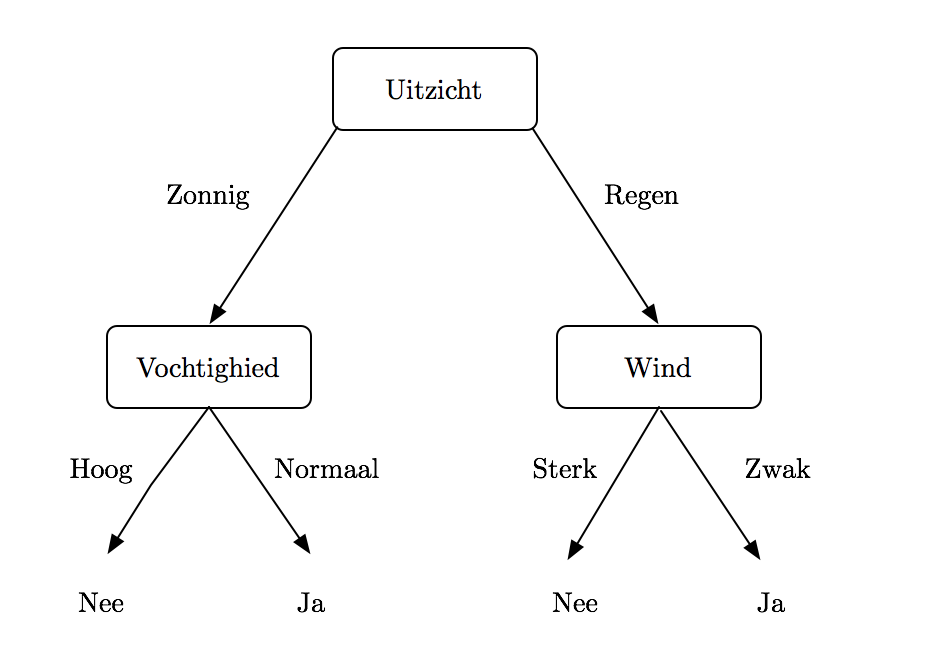
\includegraphics[width=8cm]{decisiontree}
  \captionof{figure}{Voorbeeld van een beslissingsboom}
  \label{fig:beslissingsboom}
\end{center}
